In diesem Kapitel werden die Messresultate dokumentiert.

Die verwendeten Python-Skripte zur Berechnung der statistischen Grössen und zum Plotten der Diagramme befinden sich im
Anhang~\ref{sec:python_analyze}.

Das verwendete \acrfull{dso} ist ein Rohde \& Schwarz RTB2004 1.25 GSa/s.

\subsection{Elektrische Messungen}

In diesem Teilkapitel werden die Messresultate dokumentiert, welche rein elektrisch (also ohne optischen Teil) erfasst
wurde.

Die Zeitmessungen werden von \lstinline|IC1| (siehe Abbildung~\ref{fig:tdc_ele_signal}) durchgeführt und von der
Firmware, welche auf dem Nucleo Board \lstinline|U1| (siehe Abbildung~\ref{fig:nucleo_board}) getriggert und ausgelesen.

\subsubsection{GPIO Toggle mit HAL}\label{sec:gpio_toggle_with_hal}

Als erstes wird gemessen, wie lange es für die \acrshort{cpu} der \acrshort{mcu} dauert mittels \acrfull{hal} - Library
\cite{st2020stm32f0_hal} zwei \acrshort{gpio}-Pins zu schalten.

In Code~\ref{code:gpio_toggle_with_hal} ist die Firmware-Implementation dazu gezeigt.

\lstinputlisting[language={C}, label={code:gpio_toggle_with_hal}, caption={\acrshort{gpio} Toggle mit \acrshort{hal}}]{sourcecode/gpio_toggle_with_hal.c}

Der \acrshort{tdc} misst also die Zeit zwischen Zeile 15 und 16 in Code~\ref{code:gpio_toggle_with_hal}. Dazu wird der
STOP-Pin des \acrshort{tdc} via \lstinline|SW1| mit \lstinline|stop_ele| verbunden. Der Kabelanschluss \lstinline|J3|
wird kurzgeschlossen. Siehe Abbildung~\ref{fig:tdc_ele_signal}.

Via \acrshort{uart} wurden 2000 Messwerte erfasst. Ein Ausschnitt davon ist in Code \ref{code:gpio_toggle_with_hal_log}
gezeigt. Die restlichen Daten befinden sich im elektronischen Anhang.

\lstinputlisting[language={}, label={code:gpio_toggle_with_hal_log}, caption={\acrshort{gpio} Toggle mit \acrshort{hal}}]{sourcecode/gpio_toggle_with_hal_log.txt}

Arithmetischer Mittelwert und Standardabweichung sind in Formel \ref{eq:gpio_toggle_with_hal} aufgeführt.

\begin{equation}\label{eq:gpio_toggle_with_hal}
    \begin{split}
        \overline{ToF} &= 6'375'888~ps\\
        \sigma         &= 1'059~ps
    \end{split}
\end{equation}
\myequations{\acrshort{gpio} Toggle mit \acrshort{hal}}

Da die \acrshort{cpu} mit 8~MHz läuft, lässt sich daraus schliessen, dass ein Pin-Toggle mit \acrshort{hal} ca. 50
\acrshort{cpu}-Cycles benötigt. Dies erscheint plausibel.

Histogramm und Boxplot sind in Abbildung~\ref{fig:gpio_toggle_with_hal_histogram} bzw.
\ref{fig:gpio_toggle_with_hal_boxplot} dargestellt.

\begin{figure}[H]
    \centering
    \includesvg[width=0.8\textwidth]{graphics/gpio_toggle_with_hal_histogram.svg}
    \caption{\acrshort{gpio} Toggle mit \acrshort{hal} - Histogramm}\label{fig:gpio_toggle_with_hal_histogram}
\end{figure}

\begin{figure}[H]
    \centering
    \includesvg[width=0.8\textwidth]{graphics/gpio_toggle_with_hal_boxplot.svg}
    \caption{\acrshort{gpio} Toggle mit \acrshort{hal} - Boxplot}\label{fig:gpio_toggle_with_hal_boxplot}
\end{figure}

Um die Resultate des \acrshort{tdc} zu validieren, wurde dieselbe Messung auch mittels \acrfull{dso} durchgeführt. Die
Messungen sind in Abbildung~\ref{fig:gpio_toggle_with_hal_dso} und \ref{fig:gpio_toggle_with_hal_dso_zoom} dargestellt.

\begin{figure}[H]
    \centering
    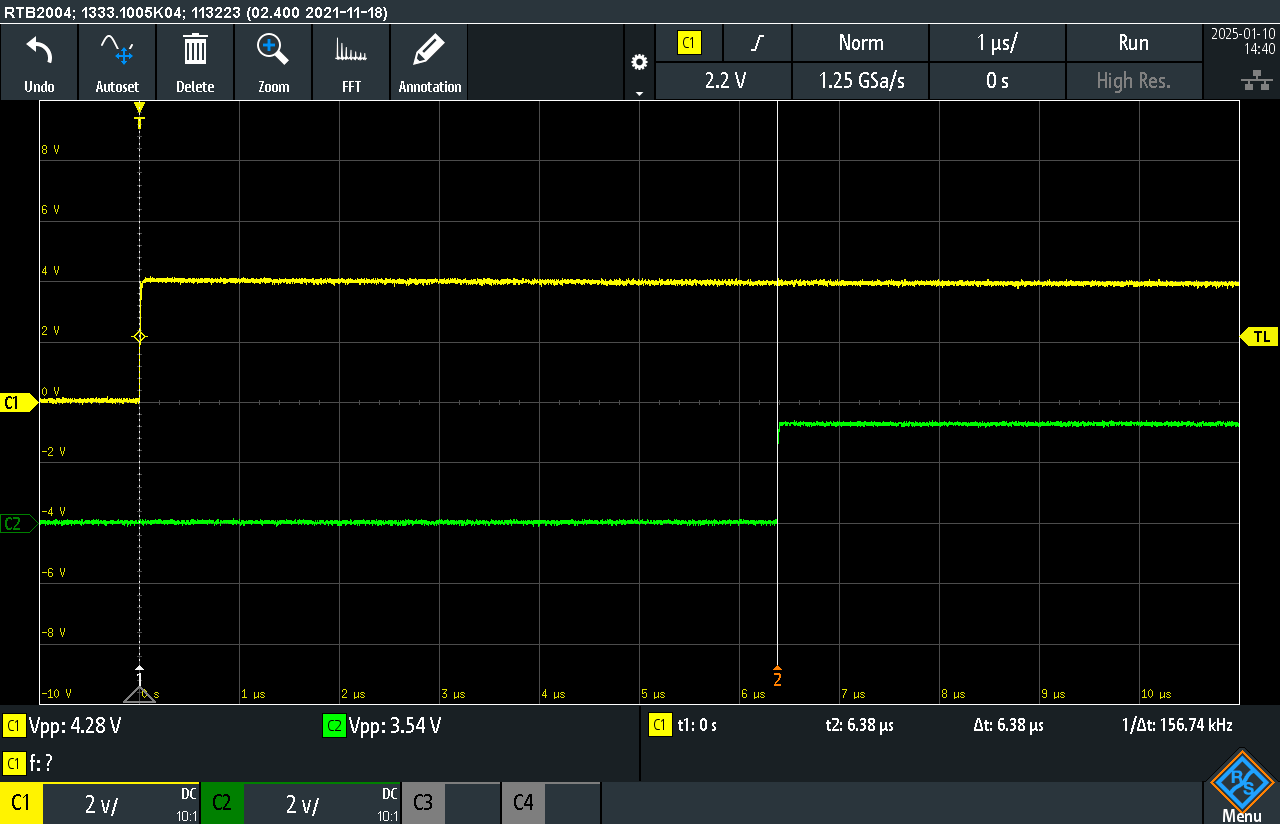
\includegraphics[width=0.8\textwidth]{graphics/gpio_toggle_with_hal_dso.png}
    \caption{\acrshort{gpio} Toggle mit \acrshort{hal} - \acrshort{dso}}\label{fig:gpio_toggle_with_hal_dso}
\end{figure}

\begin{figure}[H]
    \centering
    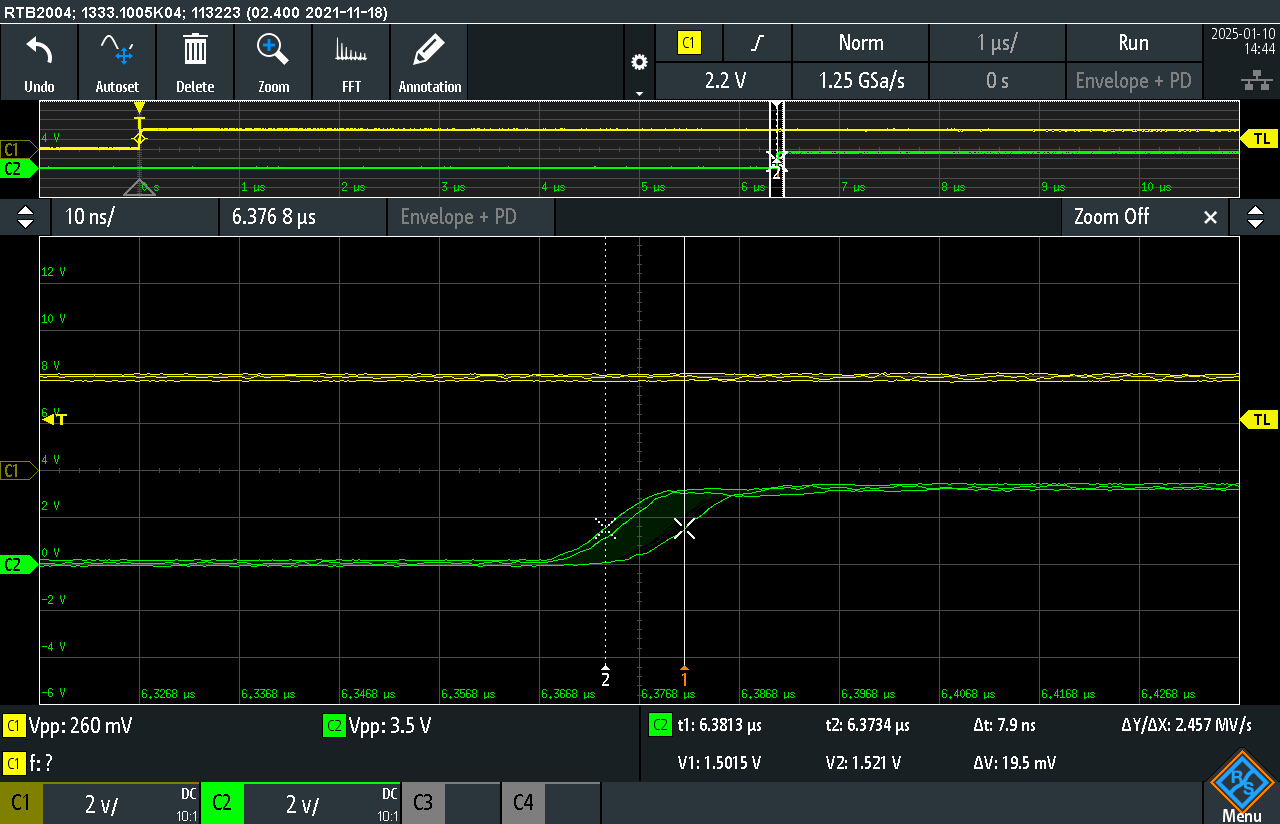
\includegraphics[width=0.8\textwidth]{graphics/gpio_toggle_with_hal_dso_zoom.png}
    \caption{\acrshort{gpio} Toggle mit \acrshort{hal} - \acrshort{dso} (Zoom)}\label{fig:gpio_toggle_with_hal_dso_zoom}
\end{figure}

\subsubsection{GPIO Toggle ohne HAL}\label{sec:gpio_toggle_without_hal}

Als nächstes wird gemessen wie lange es für die \acrshort{cpu} der \acrshort{mcu} dauert mit direktem Register-Zugriff
(via Pointer; ohne \acrshort{hal}-Library) zwei \acrshort{gpio}-Pins zu schalten.

In Code~\ref{code:gpio_toggle_without_hal} ist die Firmware-Implementation dazu gezeigt.

\lstinputlisting[language={C}, label={code:gpio_toggle_without_hal}, caption={\acrshort{gpio} Toggle ohne \acrshort{hal}}]{sourcecode/gpio_toggle_without_hal.c}

Der \acrshort{tdc} misst also die Zeit zwischen Zeile 15 und 16 in Code~\ref{code:gpio_toggle_without_hal}. Dazu wird,
wie in Kapitel \ref{sec:gpio_toggle_with_hal}, der STOP-Pin des \acrshort{tdc} via \lstinline|SW1| mit
\lstinline|stop_ele| verbunden. Der Kabelanschluss \lstinline|J3| wird kurzgeschlossen. Siehe
Abbildung~\ref{fig:tdc_ele_signal}.

Via \acrshort{uart} wurden 2000 Messwerte erfasst. Ein Ausschnitt davon ist in Code
\ref{code:gpio_toggle_without_hal_log} gezeigt. Die restlichen Daten befinden sich im elektronischen Anhang.

\lstinputlisting[language={}, label={code:gpio_toggle_without_hal_log}, caption={\acrshort{gpio} Toggle ohne \acrshort{hal}}]{sourcecode/gpio_toggle_without_hal_log.txt}

Arithmetischer Mittelwert und Standardabweichung sind in Formel \ref{eq:gpio_toggle_without_hal} aufgeführt.

\begin{equation}\label{eq:gpio_toggle_without_hal}
    \begin{split}
        \overline{ToF} &= 1'377'773~ps\\
        \sigma         &= 402~ps
    \end{split}
\end{equation}
\myequations{\acrshort{gpio} Toggle ohne \acrshort{hal}}

Da die \acrshort{cpu} mit 8~MHz läuft, lässt sich daraus schliessen, dass ein Pin-Toggle ohne \acrshort{hal} ca. 10
\acrshort{cpu}-Cycles benötigt. Dies erscheint plausibel.

Histogramm und Boxplot sind in Abbildung~\ref{fig:gpio_toggle_without_hal_histogram} bzw.
\ref{fig:gpio_toggle_without_hal_boxplot} dargestellt.

\begin{figure}[H]
    \centering
    \includesvg[width=0.8\textwidth]{graphics/gpio_toggle_without_hal_histogram.svg}
    \caption{\acrshort{gpio} Toggle ohne \acrshort{hal} - Histogramm}\label{fig:gpio_toggle_without_hal_histogram}
\end{figure}

\begin{figure}[H]
    \centering
    \includesvg[width=0.8\textwidth]{graphics/gpio_toggle_without_hal_boxplot.svg}
    \caption{\acrshort{gpio} Toggle ohne \acrshort{hal} - Boxplot}\label{fig:gpio_toggle_without_hal_boxplot}
\end{figure}

Um die Resultate des \acrshort{tdc} zu validieren, wurde dieselbe Messung auch mittels \acrfull{dso} durchgeführt. Die
Messungen sind in Abbildung~\ref{fig:gpio_toggle_without_hal_dso} und \ref{fig:gpio_toggle_without_hal_dso_zoom}
dargestellt.

\begin{figure}[H]
    \centering
    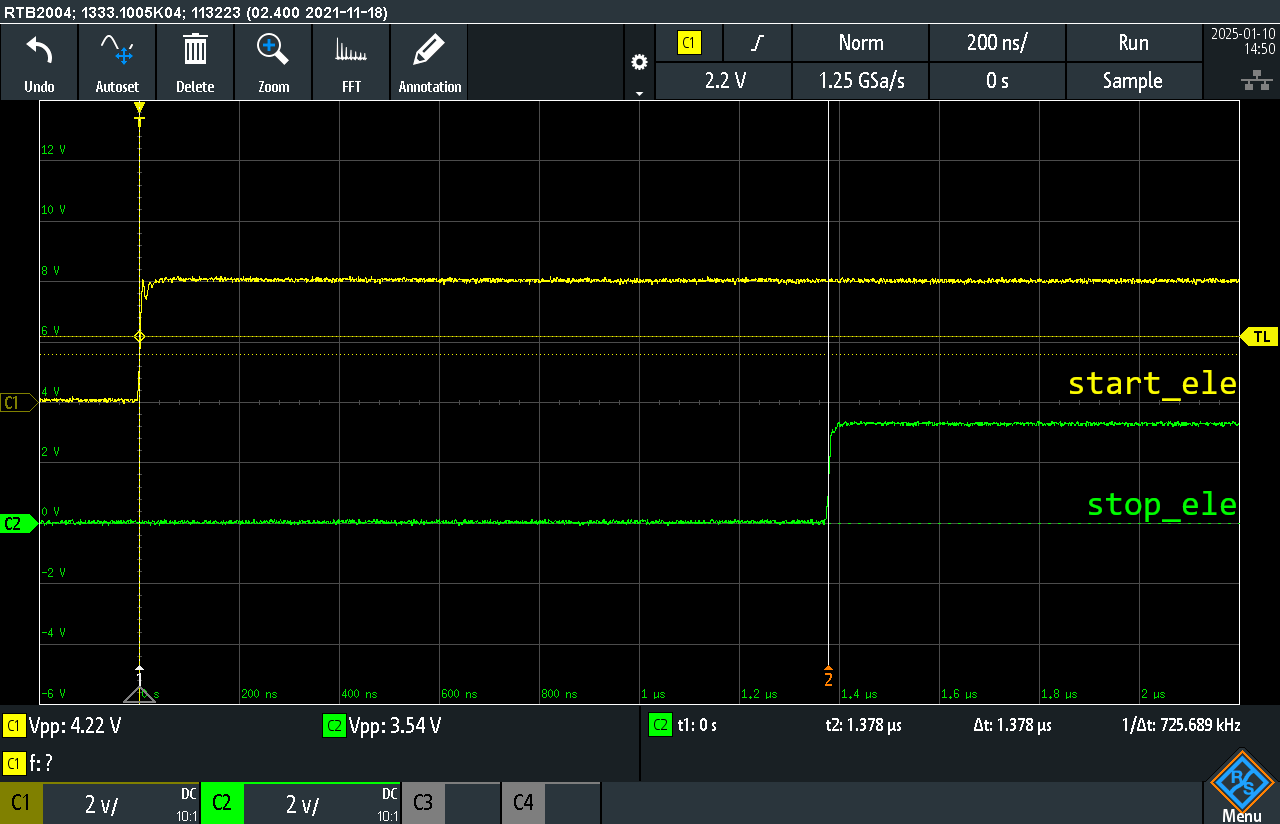
\includegraphics[width=0.8\textwidth]{graphics/gpio_toggle_without_hal_dso.png}
    \caption{\acrshort{gpio} Toggle ohne \acrshort{hal} - \acrshort{dso}}\label{fig:gpio_toggle_without_hal_dso}
\end{figure}

\begin{figure}[H]
    \centering
    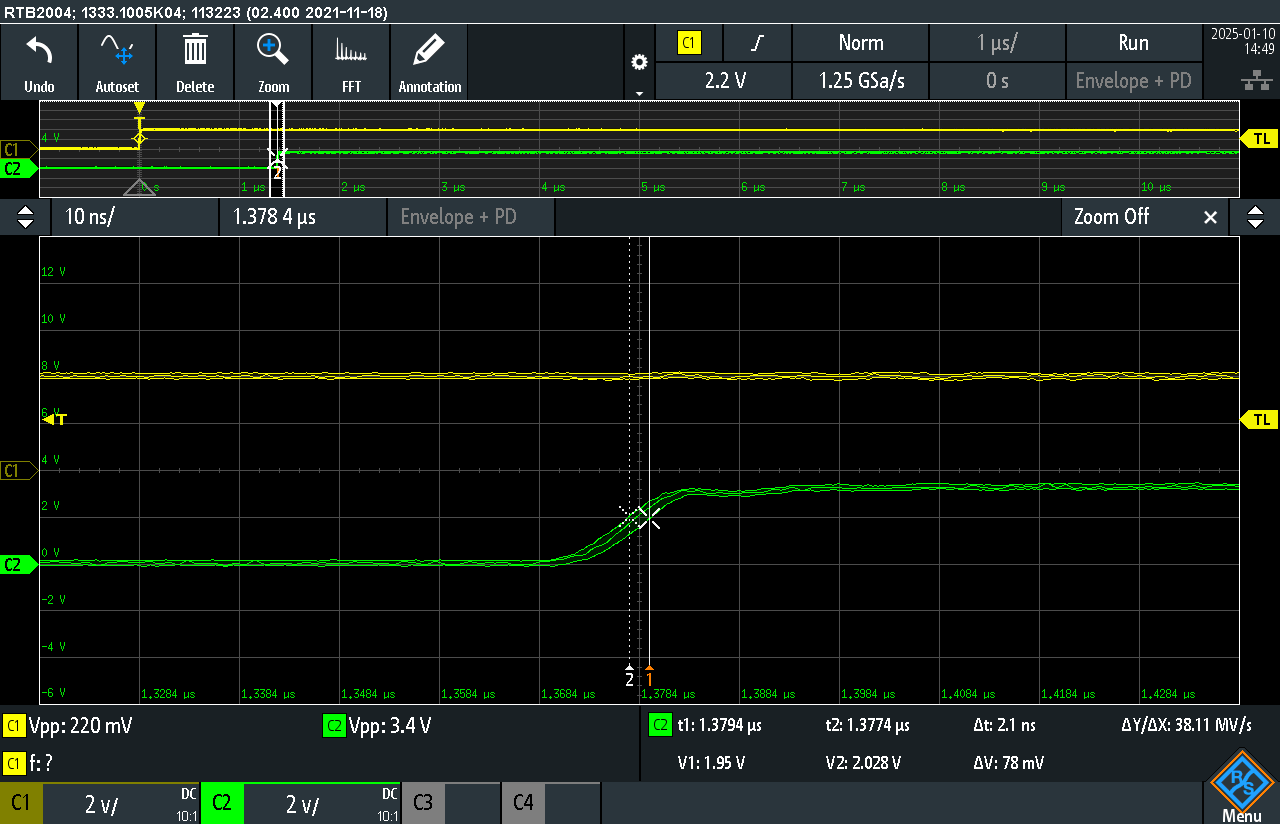
\includegraphics[width=0.8\textwidth]{graphics/gpio_toggle_without_hal_dso_zoom.png}
    \caption{\acrshort{gpio} Toggle ohne \acrshort{hal} - \acrshort{dso} (Zoom)}\label{fig:gpio_toggle_without_hal_dso_zoom}
\end{figure}

\subsubsection{Unterschiedliche Kabellängen}\label{sec:different_cable_lengths}

Für diese Messung wird dasselbe Setup wie in Kapitel \ref{sec:gpio_toggle_without_hal} verwendet.

Anstelle eines Kurzschlusses von \lstinline|J3| (siehe Abbildung \ref{fig:tdc_ele_signal}) werden nun verschiedene
Kabellängen angeschlossen.

Es hat sich herausgestellt, dass eine kreisförmige Anordnung des Kabels wichtig ist. Denn bei einer Überlappung der
beiden Kabelenden werden kürze Zeiten gemessen. Dies hat mit der kapazitiven Kopplung zwischen den Leitern zu tun.

Die Resultate sind in Abbildung~\ref{fig:different_cable_lengths} dargestellt. Die Liste mit den Datenpunkten befindet
sich im elektronischen Anhang.

\begin{figure}[H]
    \centering
    \includesvg[width=0.9\textwidth]{graphics/different_cable_lengths.svg}
    \caption{Unterschiedliche Kabellängen}\label{fig:different_cable_lengths}
\end{figure}

Die arithmetischen Mittelwerte und Standardabweichungen sind in Tabelle \ref{tab:different_cable_lengths} aufgeführt.

\begin{table}[H]
    \mytable
        {|l|l|l|}
        {\textbf{Länge} & \textbf{Mittelwert} & \textbf{Standardabweichung}}
        {\length & \mean & \stddev}
        {tables/different_cable_lengths.csv}
    \caption{Unterschiedliche Kabellängen}\label{tab:different_cable_lengths}
\end{table}

Die Signal-Ausbreitungsgeschwindigkeit in Kupfer beträgt ca. 2/3 der Lichtgeschwindigkeit
\cite{firewallcx2025propagationdelay}. Um die Resultate in Tabelle \ref{tab:different_cable_lengths} zu validieren,
rechnen wir wie in Formel \ref{eq:cable_length} gezeigt, auf die Kabellänge zurück. Die Laufzeit bei 0~m wird dabei
abgezogen, um die Verzögerung zu kompensieren, welche durch das Schalten der \acrshort{gpio}s entsteht.

\begin{equation}\label{eq:cable_length}
    \begin{split}
        c_{cu} &\approx \frac{2}{3} \cdot c_0 = \frac{2}{3} \cdot 299'792'458~\frac{m}{s} \approx 200'000'000~\frac{m}{s}\\
        ToF_{n} &= ToF_{n_{abs}} - ToF_{0}\\
        l_{n}   &= ToF_{n} \cdot c_{cu}
    \end{split}
\end{equation}
\myequations{Zurückrechnen auf Kabellänge}

Die Resultate sind in Tabelle \ref{tab:different_cable_lengths_calc} dargestellt.

\begin{table}[H]
    \mytable
        {|l|l|l|}
        {\textbf{Tatsächliche Länge} & \textbf{ToF\_n} & \textbf{Zurückgerechnete Länge}}
        {\reallength & \tofn & \calclength}
        {tables/different_cable_lengths_calc.csv}
    \caption{Kabellängen zurückgerechnet}\label{tab:different_cable_lengths_calc}
\end{table}

Es fällt auf, dass die Resultate nicht genau übereinstimmen. Dies hat mehrere Ursachen: Die Ausbreitungsgeschwindigkeit
ist nicht genau bekannt und die tatsächlichen Kabellängen wurden nicht genau gemessen.

%TODO Lets challenge this. Maybe 2/3 c is wrong for pure copper and it should be something like 95\% ?

Es ist jedoch eine klare Korrelation zu erkennen.

\subsubsection{Mode 1 vs. Mode 2}

%TODO: Evtl. Beschreibung der TDC-Modi in ein anderes Kapitel verschieben. z.B. Theorie/TDC?

Der TDC7200 unterstützt zwei Modi mit unterschiedlichen Messbereichen \cite{ti2016tdc7200_datasheet}:

\begin{itemize}
    \item Mode 1: 12~ns bis 500~ns
    \item Mode 2: 250~ns bis 8~ms
\end{itemize}

Im Mode~1 wird nur der interne Ring-Oszillator des \acrshort{tdc} verwendet. Siehe dazu Abbildung~\ref{fig:tdc_mode1}.

\begin{figure}[H]
    \centering
    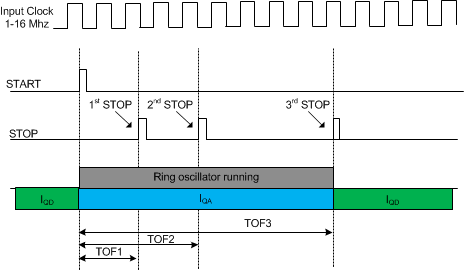
\includegraphics[width=0.6\textwidth]{graphics/tdc_mode1.png}
    \caption[\acrshort{tdc} Mode 1]{\acrshort{tdc} Mode 1 \cite{ti2016tdc7200_datasheet}}\label{fig:tdc_mode1}
\end{figure}

Im Mode~2, um längere Zeiten messen zu können, wir zusätzlich der externe Clock des \acrshort{tdc} verwendet. Siehe dazu
Abbildung~\ref{fig:tdc_mode2}.

\begin{figure}[H]
    \centering
    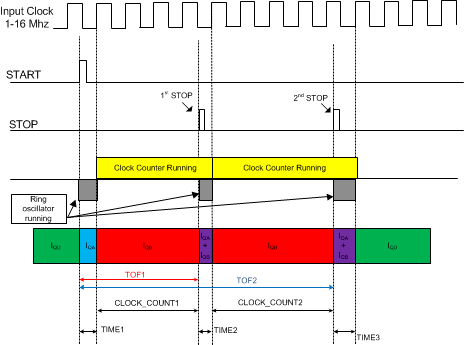
\includegraphics[width=0.6\textwidth]{graphics/tdc_mode2.png}
    \caption[\acrshort{tdc} Mode 2]{\acrshort{tdc} Mode 2 \cite{ti2016tdc7200_datasheet}}\label{fig:tdc_mode2}
\end{figure}

Die bisherigen Messungen (Kapitel~\ref{sec:gpio_toggle_with_hal}, \ref{sec:gpio_toggle_without_hal} und
\ref{sec:different_cable_lengths}) wurden im Mode~2 durchgeführt, da das Schalten der \acrshort{gpio}s mit der
\acrshort{cpu} mehr als 500~ns brauchte.

In künftigen Messungen soll das Schalten der \acrshort{gpio}s von einem Hardware-Timer der \acrshort{mcu} erledigt
werden. Damit werden Schaltzeiten von 125~ns bei 8~MHz bzw. 20.8~ns bei 48~MHz möglich sein. Es soll deshalb in diesem
Kapitel ein Vergleich der Messresultate der beiden Modi gemacht werden.

Dazu wurden drei Messungen gemacht:
\begin{enumerate}
    \item \acrshort{gpio} Toggle ohne \acrshort{hal} im Mode~2 mit Kabellänge~=~0~m (wie in Kapitel~\ref{sec:gpio_toggle_without_hal} und \ref{sec:different_cable_lengths})
    \item \acrshort{gpio} Toggle ohne \acrshort{hal} im Mode~2 mit Kabellänge~=~6~m (wie in Kapitel~\ref{sec:different_cable_lengths})
    \item Ohne GPIO Toggle Im Mode~1 mit Kabellänge~=~6~m
\end{enumerate}

Für die Messung im Mode~1 soll auf die Verzögerung durch das Schalten der \acrshort{gpio}s verzichtet werden. Dazu wird
das \lstinline|START|- und \lstinline|STOP|-Signal vom selben \acrshort{gpio}-Pin, \lstinline|start_ele|, generiert.
Dazu wird \lstinline|SW1| mit \lstinline|start_ele| verbunden (siehe Abbildung~\ref{fig:tdc_ele_signal}).

In Code~\ref{code:mode1} ist die Firmware-Implementation für eine Messung im Mode~1 gezeigt.

\lstinputlisting[language={C}, label={code:mode1}, caption={Mode 1}]{sourcecode/mode1.c}

Die Unterschiede im Vergleich zu den Messungen in Kapitel~\ref{sec:gpio_toggle_without_hal} und
\ref{sec:different_cable_lengths} sind:

\begin{itemize}
    \item Zeile 7: \acrshort{tdc} wird im Mode~1 konfiguriert (anstatt Mode~2)
    \item Zeile 15 und 23: Es wird nur der \lstinline|start_ele| Pin getoggelt (anstatt \lstinline|start_ele| und \lstinline|stop_ele| Pin)
\end{itemize}

Die Erwartung ist, dass die Differenz aus Messung~1 und Messungen~2 ungefähr dem Resultat aus Messung~3 entspricht.

Die Resultate dieser drei Messungen sind in Tabelle \ref{tab:mode1_vs_mode2} aufgeführt. Die restlichen Daten befinden
sich im elektronischen Anhang.

\begin{table}[H]
    \mytable
        {|l|l|l|}
        {\textbf{Messung} & \textbf{Mittelwert} & \textbf{Standardabweichung}}
        {\measurement & \mean & \stddev}
        {tables/mode1_vs_mode2.csv}
    \caption{Mode 1 vs. Mode 2}\label{tab:mode1_vs_mode2}
\end{table}

Die Berechnung in Formel~\ref{eq:mode1_vs_mode2} zeigt, dass die Messresultate nahe beieinander liegen.

\begin{equation}\label{eq:mode1_vs_mode2}
    \begin{split}
        \Delta Mode~2 &= 1'403'224~ps - 1'378'222~ps = 25'001~ps\\
        Mode~1        &= 25'145~ps
    \end{split}
\end{equation}
\myequations{Mode 1 vs. Mode 2}

Es kann also davon ausgegangen werden, dass Mode~1 und Mode~2 im Firmware-Treiber korrekt implementiert wurden.

Bemerkung: Im Firmware-Treiber (siehe Anhang~\ref{sec:tdc_driver}) kann für beide Modi dieselbe Funktion
\lstinline|TDC_read_result()| verwendet werden. Für Mode~1 vereinfacht sich die Berechnung, weil \lstinline|TIME2|~=~0
und \lstinline|CLOCK_COUNT1|~=~0.

\subsubsection{Timer Output}\label{sec:timer_output}

In Kapitel~\ref{sec:gpio_toggle_with_hal} und \ref{sec:gpio_toggle_without_hal} wurge gezeigt, dass es einige
\acrshort{cpu}-Cycles dauert, um  mittels Software, also mit \acrshort{cpu}-Instruktionen, \acrshort{gpio}s zu toggeln.

Eine schnellere Methode ist es, das Toggeln der \acrshort{gpio}s von der Hardware-Peripherie der \acrshort{mcu}
erledigen zu lassen. Dazu eignen sich Hardware-Timer.

In Abbildung \ref{fig:clock_config_default} ist die default Clock-Configuration des Nucleo-Boards gezeigt.

\begin{figure}[H]
    \centering
    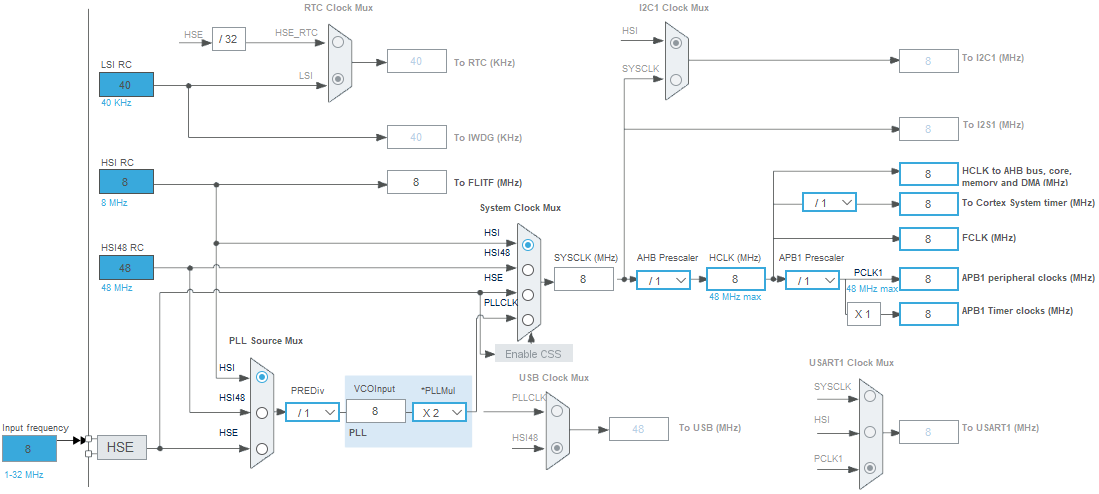
\includegraphics[width=0.9\textwidth]{graphics/clock_config_default.png}
    \caption{Default Clock-Configuration}\label{fig:clock_config_default}
\end{figure}

Per default wird der \acrfull{hsi} Clock mit 8~MHz verwendet. Damit sollte es mit Hardware-Timer möglich sein, zwei
\acrshort{gpio}s zu schalten mit einer Verzögerung gemäss Formel~\ref{eq:gpio_schalten_zeit}.

\begin{equation}\label{eq:gpio_schalten_zeit}
    t = \frac{1}{8~MHz} = 125~ns
\end{equation}
\myequations{\acrshort{gpio}-Schalten Verzögerungszeit}

Dazu werden Kanal \lstinline|CH1| und \lstinline|CH4| des Hardware-Timers \lstinline|TIM1| im Output Compare Match Modus
verwendet. Die zugeordneten \acrshort{gpio}-Pins sind \lstinline|start_ele| bzw. \lstinline|stop_ele|.

Erreicht der 16~bit Timer den Wert \lstinline|32'000| wird \lstinline|start_ele| auf High geschalten. Beim Erreichen des
Werts \lstinline|32'001| wird \lstinline|stop_ele| auf High geschalten.

Der \acrshort{tdc} wird in Mode 1 konfiguriert. Der STOP-Pin des \acrshort{tdc} wird via \lstinline|SW1| mit
\lstinline|stop_ele| verbunden. Der Kabelanschluss \lstinline|J3| wird kurzgeschlossen. Siehe
Abbildung~\ref{fig:tdc_ele_signal}.

In Code~\ref{code:timer_output} ist die Firmware-Implementation dazu gezeigt.

\lstinputlisting[language={C}, label={code:timer_output}, caption={\acrshort{gpio} Toggle mit Timer-Output}]{sourcecode/timer_output.c}

Der gemessene arithmetische Mittelwert und die Standardabweichung sind in Formel~\ref{eq:timer_output} aufgeführt.  Die
Liste mit den Datenpunkten befindet sich im elektronischen Anhang.

\begin{equation}\label{eq:timer_output}
    \begin{split}
        \overline{ToF} &=128'108~ps\\
        \sigma         &= 81~ps
    \end{split}
\end{equation}
\myequations{\acrshort{gpio} Toggle mit Timer-Output}

Erwartungsgemäss dauert das Schalten der \acrshort{gpio}s ca. 125~ns. Die Standardabweichung ist aufgrund der kleineren
Anzahl an Clock-Cycles tiefer als in den bisherigen Kapiteln.

\subsubsection{Unterschiedliche Clock-Konfigurationen}

In diesem Teilkapitel werden Messungen mit demselben Setup wie in Kapitel~\ref{sec:timer_output} durchgeführt.

Es werden die arithmetischen Mittelwerte und die Standardabweichungen verschiedener Clock-Quellen des Nucleo-Boards
verglichen. Es werden drei Messungen gemacht:

\begin{enumerate}
    \item \acrshort{hsi}: 8~MHz (wie in Kapitel~\ref{sec:timer_output})
    \item \acrshort{hsi} mit \acrshort{pll}: 16~MHz
    \item \acrshort{hsi}48: 48~MHz
\end{enumerate}

Die Clock-Konfigurationen für Messung 2 und 3 sind in Abbildung~\ref{fig:clock_config_hsi_pll_16mhz} bzw.
\ref{fig:clock_config_hsi48_48mhz} dargestellt.

\begin{figure}[H]
    \centering
    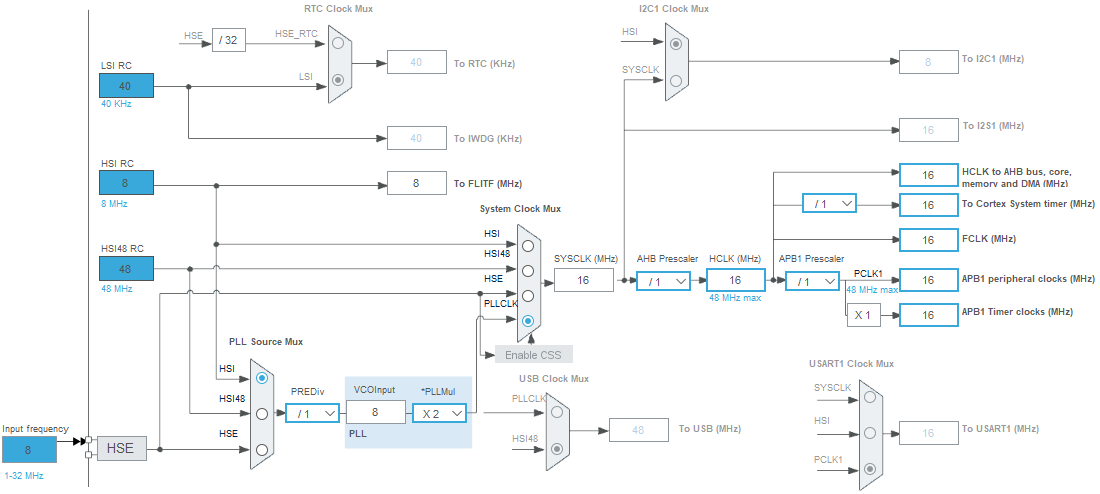
\includegraphics[width=0.9\textwidth]{graphics/clock_config_hsi_pll_16mhz.png}
    \caption{Clock-Configuration \acrshort{hsi} mit \acrshort{pll} 16~MHz}\label{fig:clock_config_hsi_pll_16mhz}
\end{figure}

\begin{figure}[H]
    \centering
    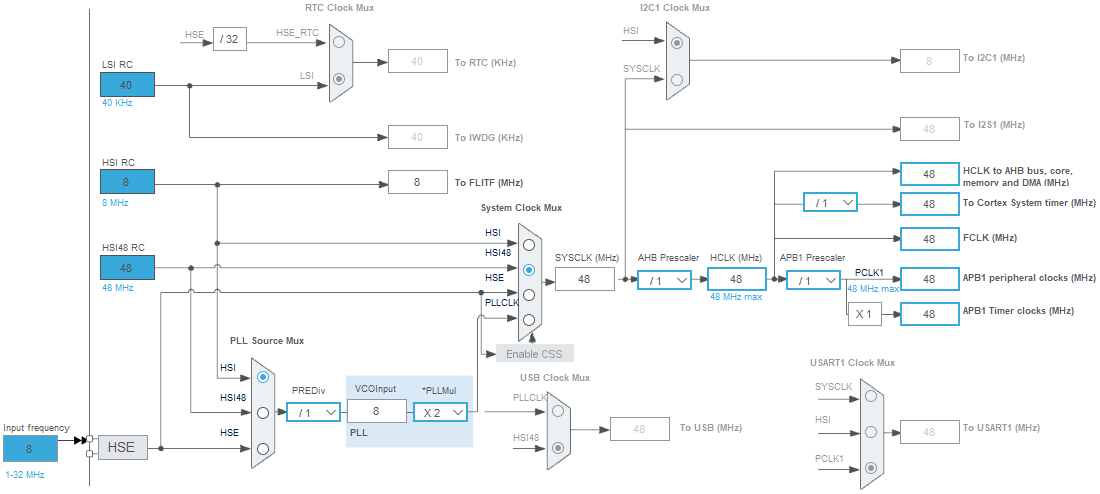
\includegraphics[width=0.9\textwidth]{graphics/clock_config_hsi48_48mhz.png}
    \caption{Clock-Configuration \acrshort{hsi}48 48~MHz}\label{fig:clock_config_hsi48_48mhz}
\end{figure}

Die arithmetischen Mittelwerte und Standardabweichungen sind in Tabelle~\ref{tab:different_clock_sources} dargestellt.
Die Liste mit den Datenpunkten befindet sich im elektronischen Anhang.

\begin{table}[H]
    \mytable
        {|l|l|l|}
        {\textbf{Messung} & \textbf{Mittelwert} & \textbf{Standardabweichung}}
        {\measurement & \mean & \stddev}
        {tables/different_clock_sources.csv}
    \caption{Unterschiedliche Clock-Quellen}\label{tab:different_clock_sources}
\end{table}

Die Resultate stimmen ungefähr mit den erwarteten Werten aus Formel~\ref{eq:gpio_schalten_zeiten} überein.

\begin{equation}\label{eq:gpio_schalten_zeiten}
    \begin{split}
        t_1 &= \frac{1}{8~MHz} = 125~ns\\
        t_2 &= \frac{1}{16~MHz} = 62.5~ns\\
        t_3 &= \frac{1}{48~MHz} = 20.8~ns
    \end{split}
\end{equation}
\myequations{\acrshort{gpio}-Schalten Verzögerungszeiten}

Im Datenblatt konnte eine Angabe zum \acrshort{pll}-Jitter gefunden werden, siehe Abbildung~\ref{fig:pll_jitter}.

\begin{figure}[H]
    \centering
    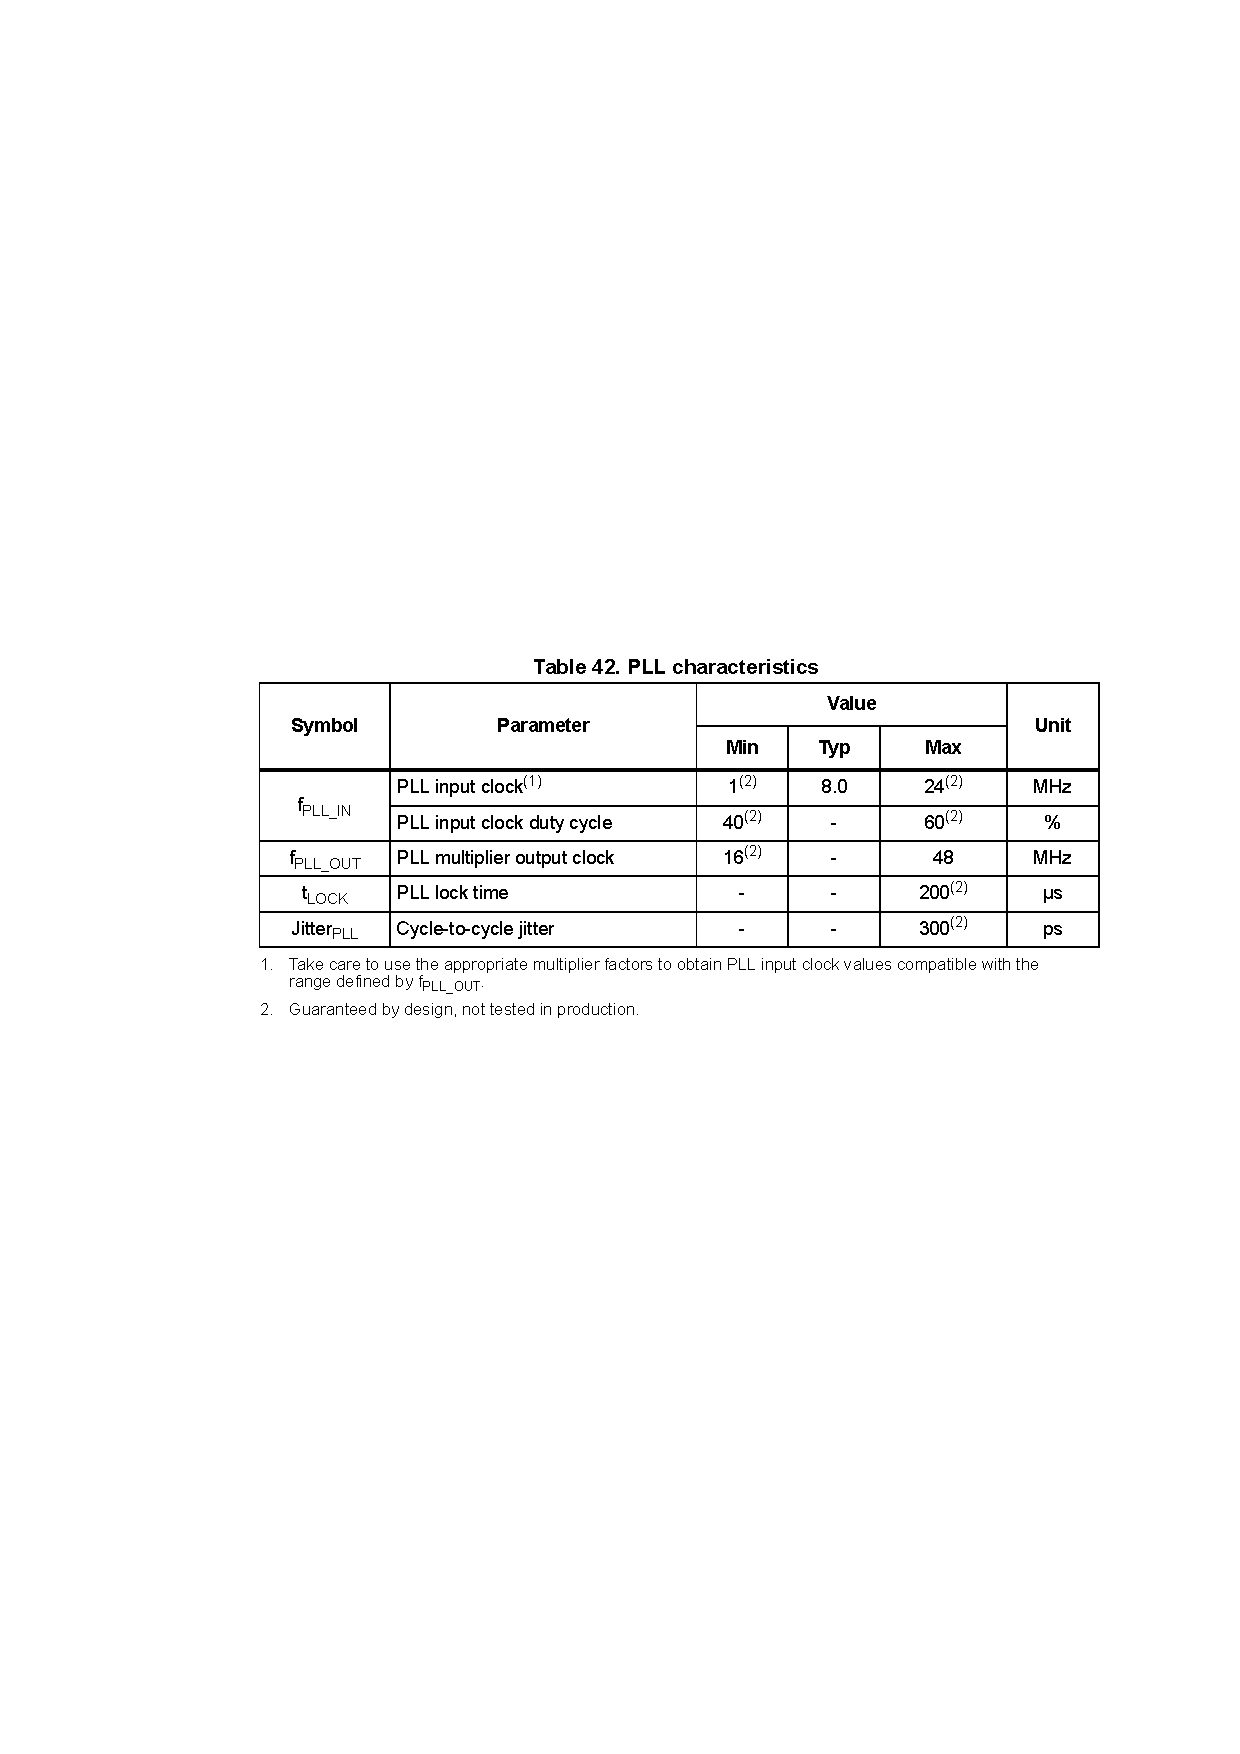
\includegraphics[width=0.8\textwidth]{graphics/pll_jitter.pdf}
    \caption[\acrshort{pll}-Jitter]{\acrshort{pll}-Jitter \cite{st2017stm32f042k6_datasheet}}\label{fig:pll_jitter}
\end{figure}

Diese Angabe ist ungefähr in derselben Grössenordnung wie die Messresultate.

\pagebreak

\subsection{Optische Messungen}

%TODO
